\subsection{UC17: Gestione profilo}
\label{sec:UC17}
\begin{figure}[!ht]
    \caption{Diagramma di UC17: Gestione profilo}
    \vspace{10px}
    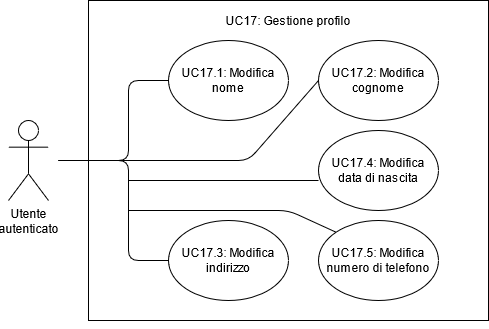
\includegraphics[scale=0.5]{../../../Images/AnalisiRequisiti/UC17}
    \centering
\end{figure}

\begin{itemize}
    \item \textbf{Descrizione:} l'utente vuole gestire il proprio profilo;
    \item \textbf{Attore Primario:} utente autenticato;
    \item \textbf{Attore Secondario:} servizio di autenticazione esterno;
    \item \textbf{Precondizione:} l'utente si trova all'interno del proprio profilo;
    \item \textbf{Postcondizione:} l'utente può modificare il proprio profilo;
    \item \textbf{Scenario Principale:}
          \begin{itemize}
              \item  l'utente decide cosa modificare tra:
                    \begin{itemize}
                        \item nome;
                        \item cognome;
                        \item indirizzo;
                        \item data di nascita;
                        \item numero di telefono.
                    \end{itemize}
          \end{itemize}
\end{itemize}

\subsubsection{UC17.1 Modifica del nome}
\label{sec:UC17.1}
\begin{itemize}
    \item \textbf{Descrizione:} l'utente vuole modificare il proprio nome relativo all'account;
    \item \textbf{Attore Primario:} utente autenticato;
    \item \textbf{Attore Secondario:} servizio di autenticazione esterno;
    \item \textbf{Precondizione:} l'utente si trova all'interno del proprio profilo;
    \item \textbf{Postcondizione:} l'utente può modificare il proprio nome.
\end{itemize}

\subsubsection{UC17.2 Modifica del cognome}
\label{sec:UC17.2}
\begin{itemize}
    \item \textbf{Descrizione:} l'utente vuole modificare il proprio cognome relativo all'account;
    \item \textbf{Attore Primario:} utente autenticato;
    \item \textbf{Attore Secondario:} servizio di autenticazione esterno;
    \item \textbf{Precondizione:} l'utente si trova all'interno del proprio profilo;
    \item \textbf{Postcondizione:} l'utente può modificare il proprio cognome.
\end{itemize}

\subsubsection{UC17.3 Modifica dell'indirizzo}
\label{sec:UC17.3}
\begin{itemize}
    \item \textbf{Descrizione:} l'utente vuole modificare il proprio indirizzo;
    \item \textbf{Attore Primario:} utente autenticato;
    \item \textbf{Attore Secondario:} servizio di autenticazione esterno;
    \item \textbf{Precondizione:} l'utente si trova all'interno del proprio profilo;
    \item \textbf{Postcondizione:} l'utente può modificare il proprio indirizzo.
\end{itemize}

\subsubsection{UC17.4 Modifica della data di nascita}
\label{sec:UC17.4}
\begin{itemize}
    \item \textbf{Descrizione:} l'utente vuole modificare la data di nascita;
    \item \textbf{Attore Primario:} utente autenticato;
    \item \textbf{Attore Secondario:} servizio di autenticazione esterno;
    \item \textbf{Precondizione:} l'utente si trova all'interno del proprio profilo;
    \item \textbf{Postcondizione:} l'utente può modificare il proprio indirizzo.
\end{itemize}

\subsubsection{UC17.5 Modifica del numero di telefono}
\label{sec:UC17.5}
\begin{itemize}
    \item \textbf{Descrizione:} l'utente vuole modificare il numero di telefono;
    \item \textbf{Attore Primario:} utente autenticato;
    \item \textbf{Attore Secondario:} servizio di autenticazione esterno;
    \item \textbf{Precondizione:} l'utente si trova all'interno del proprio profilo;
    \item \textbf{Postcondizione:} l'utente può modificare il proprio indirizzo.
\end{itemize}